\documentclass[12pt]{article} %czcionka 12
\usepackage[a4paper, total={6in, 9in}]{geometry}
\usepackage{pdfpages} %wstawianie stron z .pdf
\usepackage{graphicx} %wstawianie grafiki
\usepackage{mathptmx} %czcionka Times New Roman
\usepackage[T1]{fontenc} %encoding
\usepackage{setspace}
	\onehalfspacing %interlinia 1.5
\usepackage{ragged2e}
	\justifying
\usepackage[nottoc,numbib]{tocbibind}
\usepackage{color}
	\definecolor{Green}{rgb}{0,0.901,0}
	\definecolor{Turbo}{rgb}{0.901,0.901,0}
	\definecolor{BrightTurquoise}{rgb}{0,0.901,0.901}
	\definecolor{Persimmon}{rgb}{1,0.333,0.333}
	\definecolor{Silver}{rgb}{0.752,0.752,0.752}
\usepackage{tabularray}
\usepackage{adjustbox}

\author{Miłosz Mosur}
\author{Mateusz Ossowski}
\author{Maciej Ratajski}

\renewcommand{\figurename}{Rysunek}
\renewcommand{\contentsname}{Spis treści}
\renewcommand{\refname}{Źródła, Bibliografia}


\begin{document}
	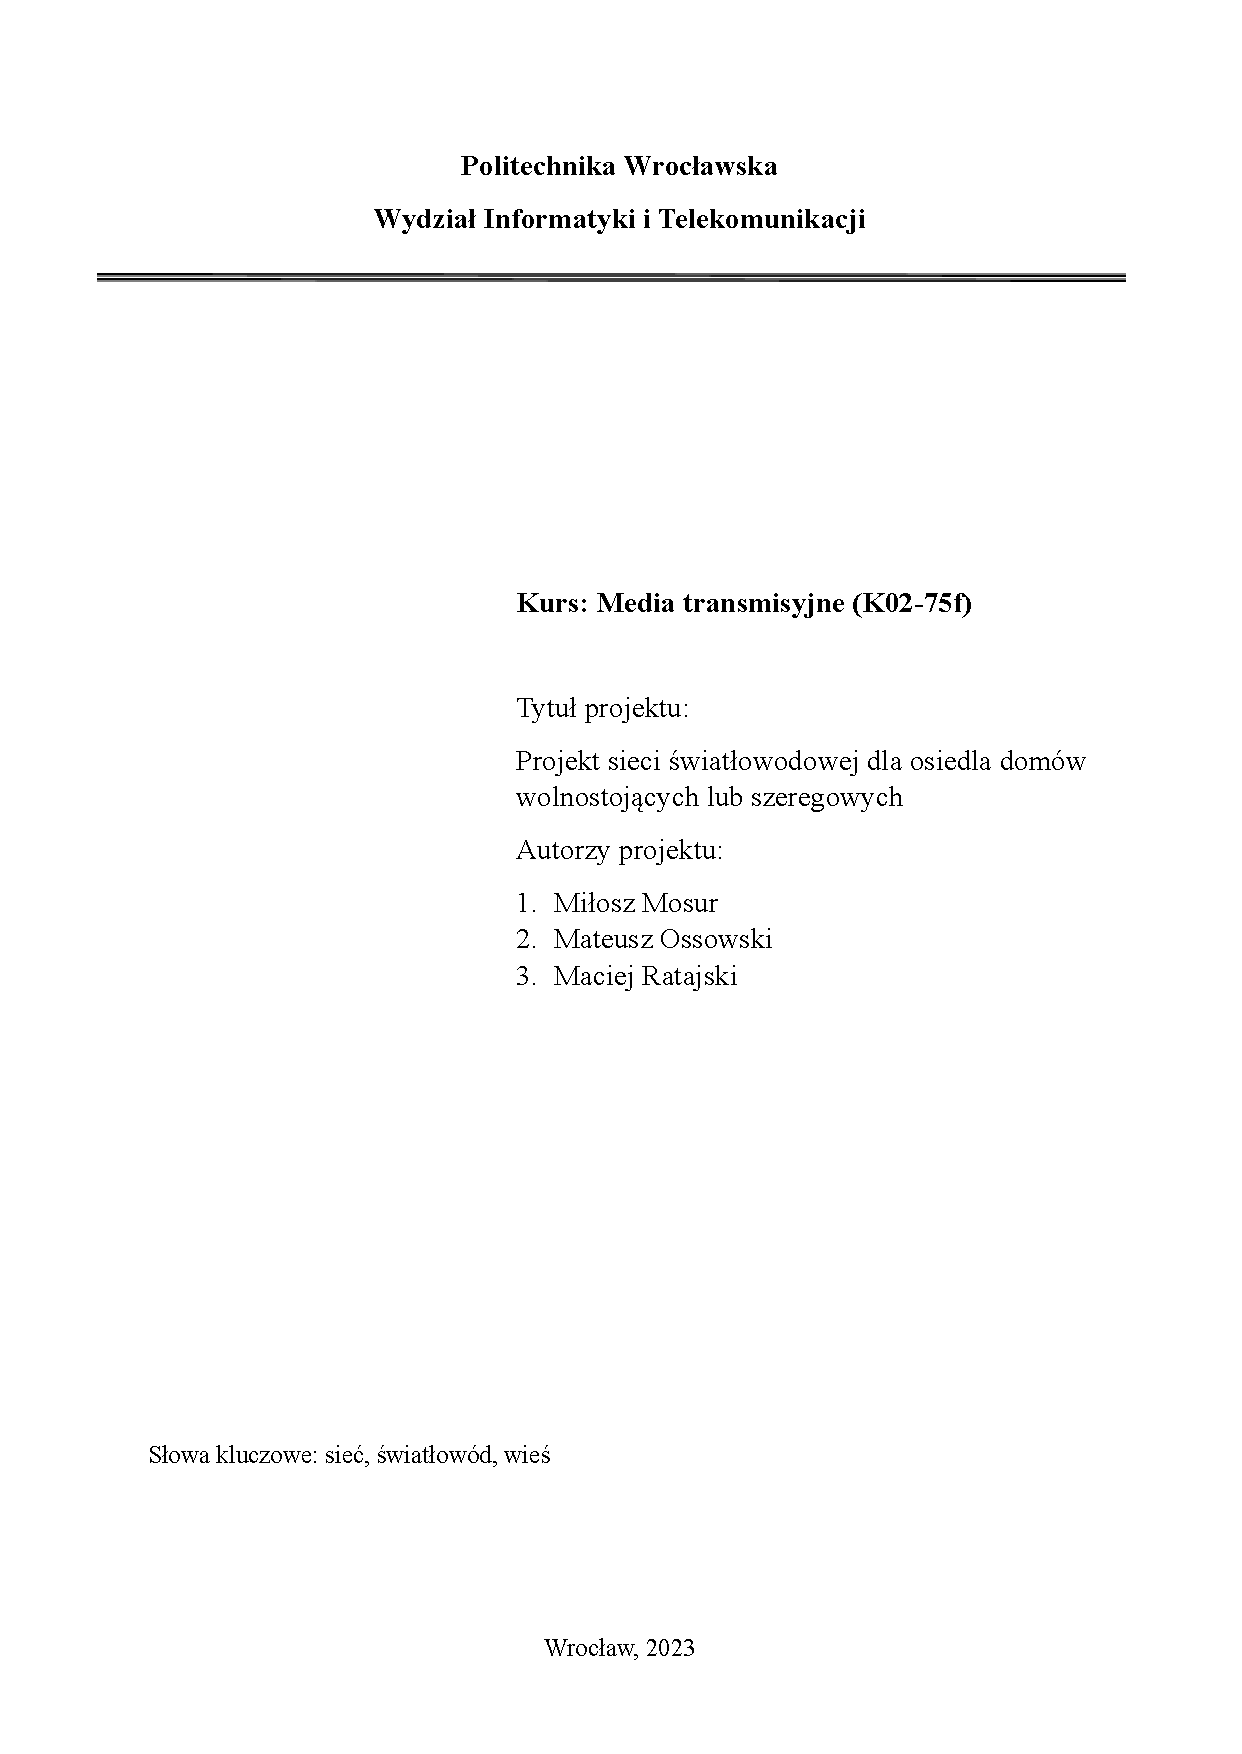
\includepdf[pages=-]{title.pdf} %strona tytułowa
	\tableofcontents
	
	\newpage
	\section{Wstęp}
		\subsection{Założenia projektu:}
\begin{itemize}
	\item \textbf{Lokalizacja}: Grabowno Wielkie (wieś), ulica, na której znajdują się domy o adresach 43-57, 80-90 (włącznie z adresami z literą a) i 121
	\item \textbf{Grupa odbiorców}: Osoby, które to nie mają dużych zapotrzebowań na szybkie łącza internetowe.
	\item \textbf{OLT}: Na wschodzie znajduję się Szkoła Podstawowa, która wydaje się być dobrym miejscem na taką infrastrukturę w tym miasteczku.
	\item \textbf{Swiatłowód}: SM (średnice 8-9 mikrometrów rdzeń, 125 mikrometrów bufor)
	\item \textbf{Przepustowość}: 1000MB/500MB per end point (budynek). Uwzględnić overbooking na poziomie około 20\%
	\item \textbf{Topologia}: P2MP
	\item \textbf{Architektura}: FTTH
	\item \textbf{System}: GPON
\end{itemize}

\newpage
\subsection{Lokalizacja}

	\begin{center}
		\begin{figure}[h!]
			\makebox[\textwidth]{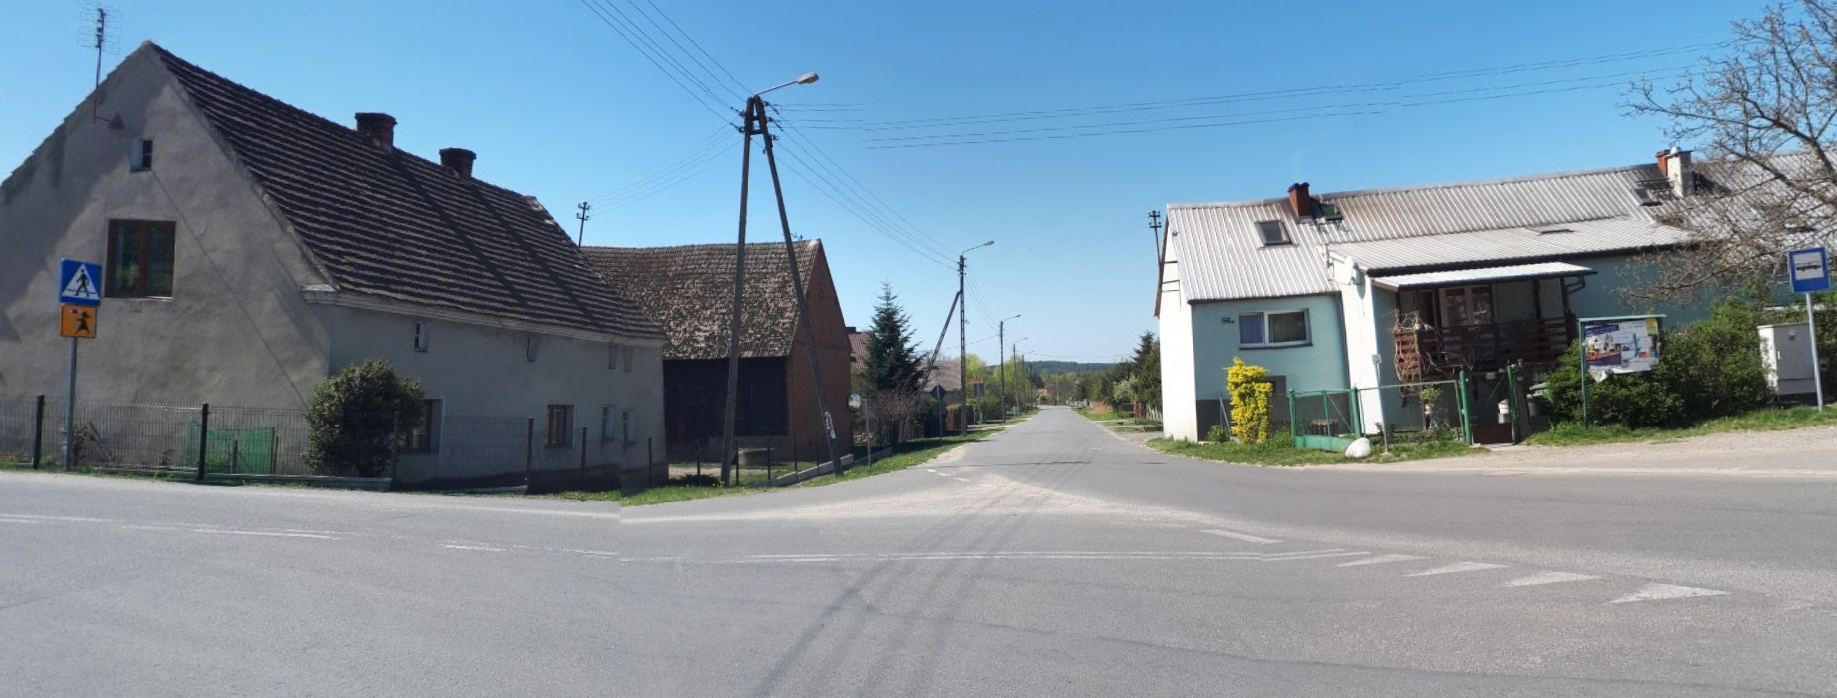
\includegraphics[width=\textwidth]{grabowno_intro.png}}
			\caption{Grabowno Wielkie}
			\label{fig:grabowno_intro}
			\begin{center}\cite{grabowno_intro}\end{center}
		\end{figure}
	
		\begin{figure}[h!]
			\makebox[\textwidth]{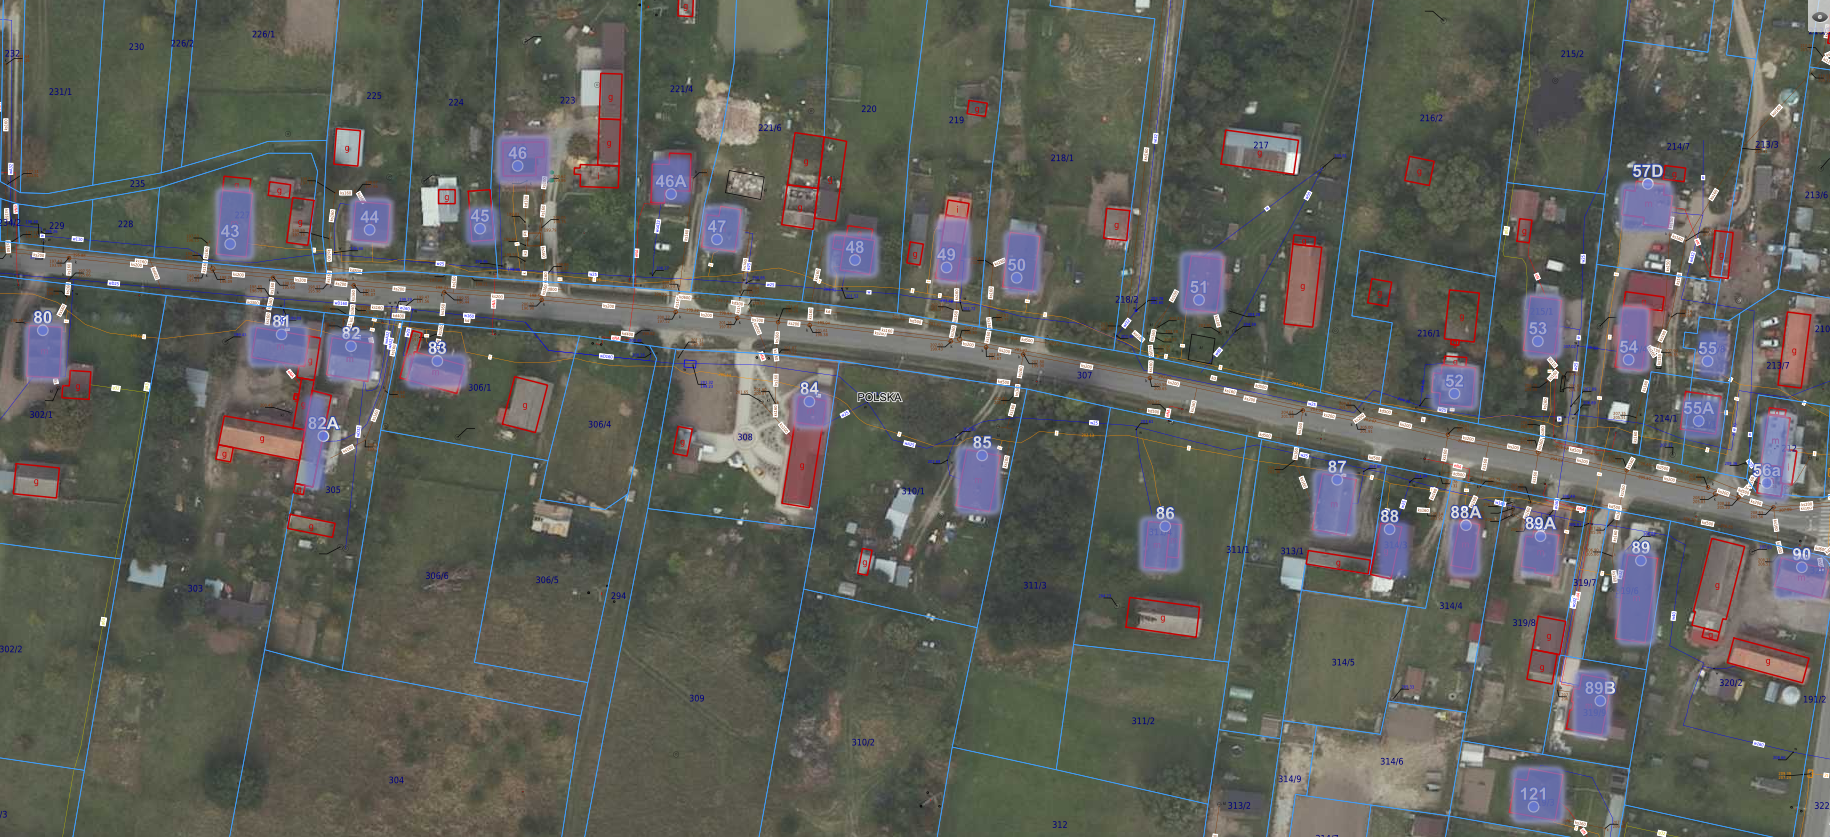
\includegraphics[width=\textwidth]{plan_intro.png}}
			\caption{Plan wsi}
			\label{fig:plan_intro}
			\begin{center}\cite{plan_intro}\end{center}
		\end{figure}
	
	\end{center}

	Numery działek mające zostać objęte siecią:
	\begin{itemize}
		\item od północnej strony ulicy numery od 43 do 57
		\item od południowej strony numery od 80 do 90 oraz 121
	\end{itemize}

	\section{Projekt logiczny}
		\subsection{Schemat}
	\begin{center}
		\begin{figure}[h!]
			\makebox[\textwidth]{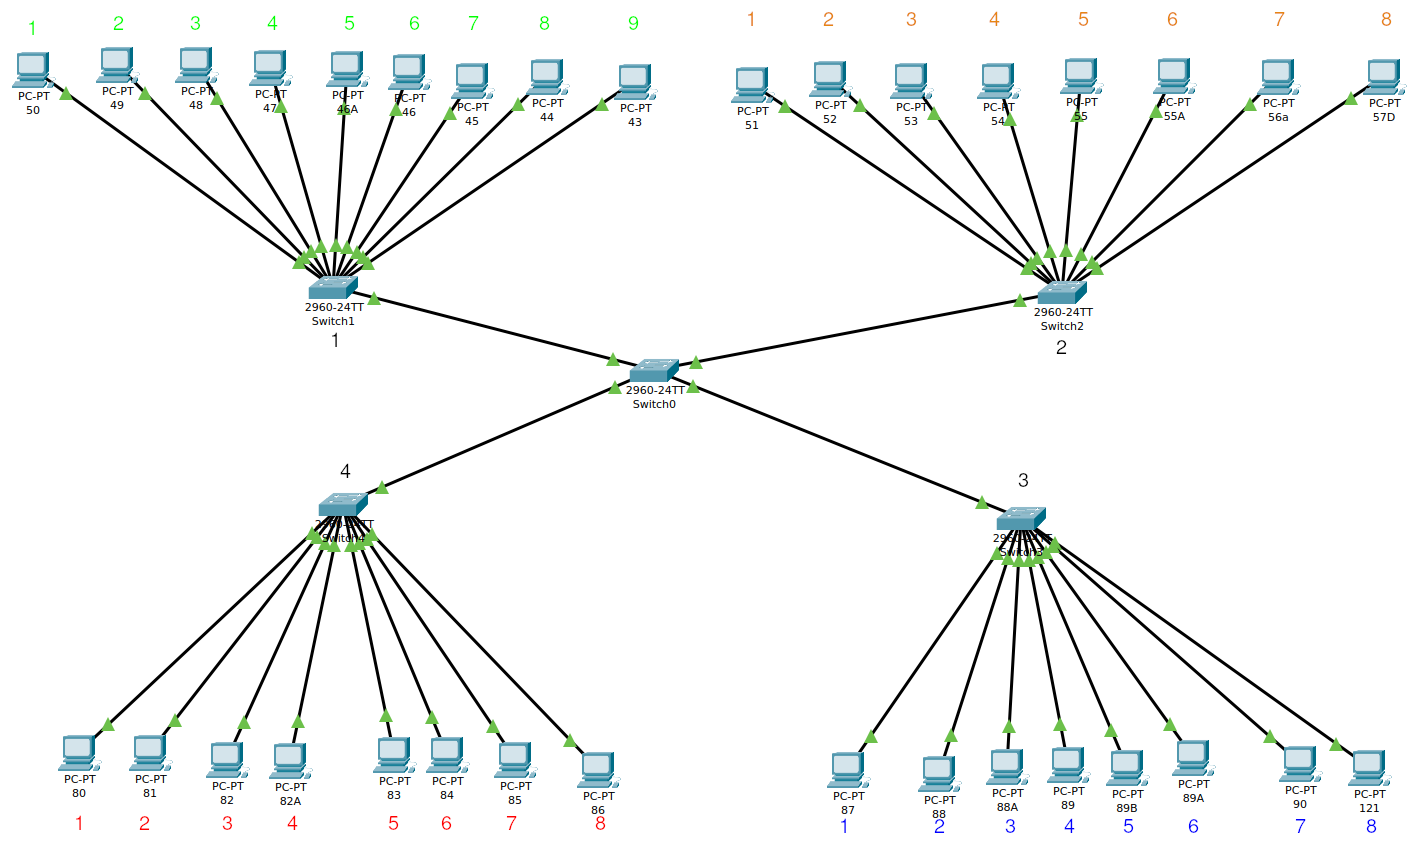
\includegraphics[width=\textwidth]{schemat_logiczny.png}}
			\caption{Schemat logiczny}
			\label{fig:schemat_logiczny}
		\end{figure}
		\begin{figure}[h!]
			\makebox[\textwidth]{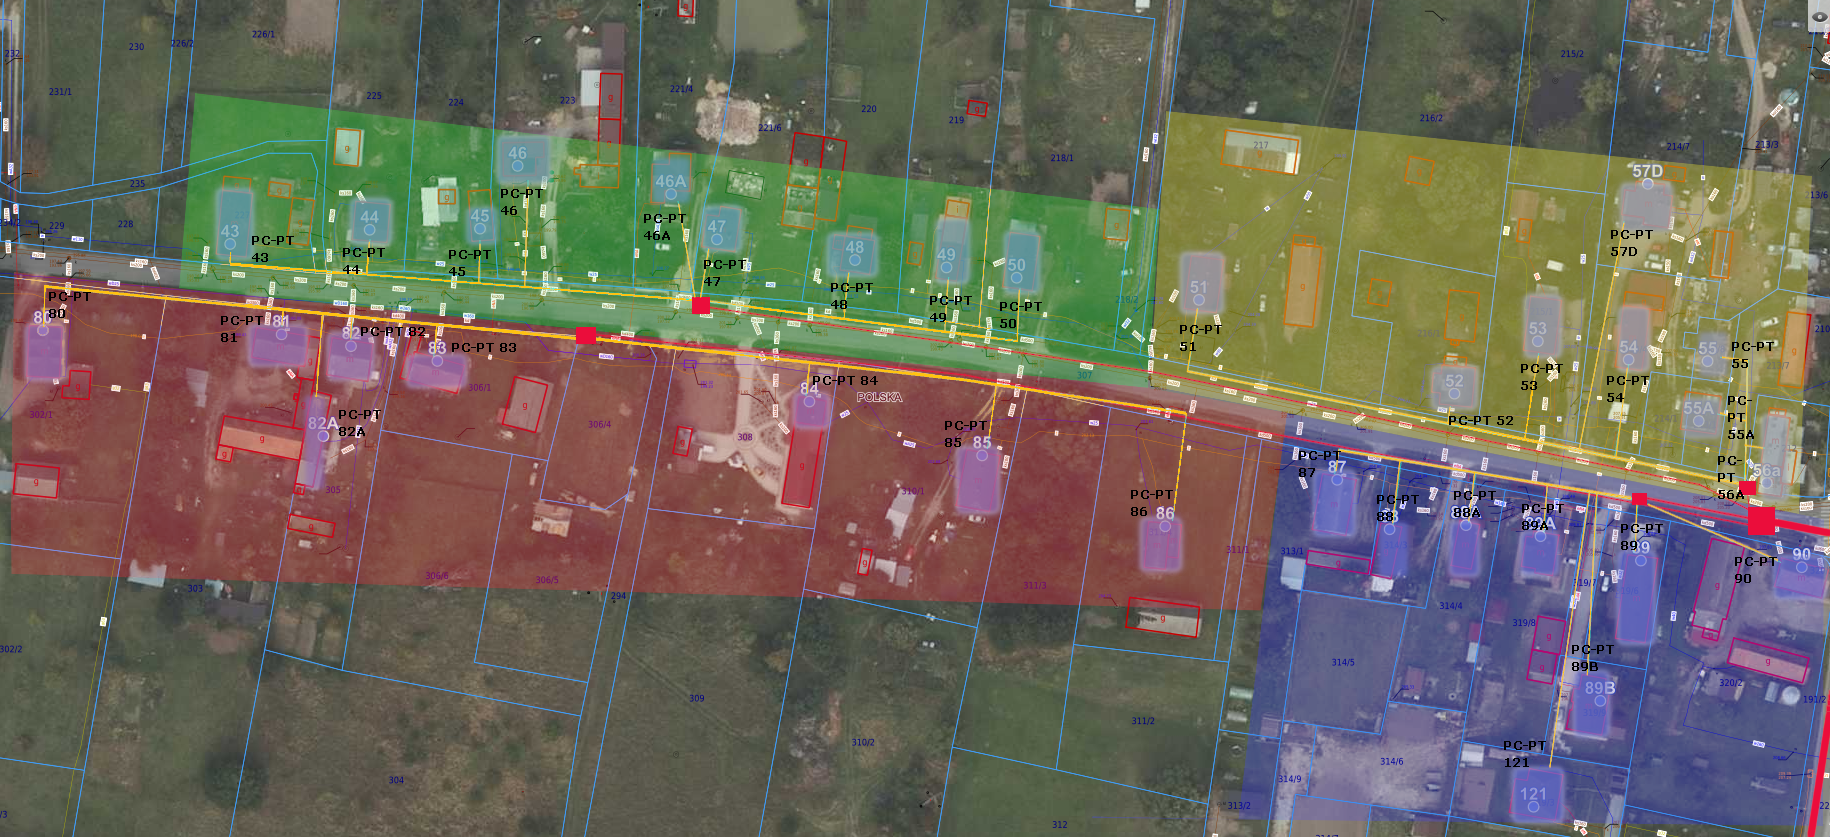
\includegraphics[width=\textwidth]{proj_gimp/proj.png}}
			\caption{Podział na podsieci na mapie fizycznej}
			\label{fig:podsieci}
		\end{figure}
	\end{center}

\subsection{Rozwiązania techologiczne}
	\paragraph{Okablowanie:}
		SM G657
	\paragraph{Złącza:}
		SC/APC (Subscriber Connector)
	\paragraph{Użyte sprzęgacze:}
		\begin{center}
			\begin{table}[htbp]
				\centering
				\begin{tabular}{|c|c|}
					\hline
					\textbf{Typ} & \textbf{ilość} \\ \hline
					1x4          & 1              \\ \hline
					1x16         & 4              \\ \hline
				\end{tabular}
			\end{table}
		\end{center}
\subsection{Podział na podsieci}
	\begin{center}
		\begin{table}[htbp]
			\centering
			\begin{tblr}{
					cells = {BrightTurquoise},
					row{2} = {c},
					column{1} = {Green},
					column{2} = {Green},
					column{3} = {Turbo},
					column{4} = {Turbo},
					column{7} = {Persimmon},
					column{8} = {Persimmon},
					cell{1}{1} = {c=2}{c},
					cell{1}{3} = {c=2}{},
					cell{1}{5} = {c=2}{},
					cell{1}{7} = {c=2}{},
					cell{3}{1} = {c},
					cell{3}{2} = {c},
					cell{4}{1} = {c},
					cell{4}{2} = {c},
					cell{5}{1} = {c},
					cell{5}{2} = {c},
					cell{6}{1} = {c},
					cell{6}{2} = {c},
					cell{7}{1} = {c},
					cell{7}{2} = {c},
					cell{8}{1} = {c},
					cell{8}{2} = {c},
					cell{9}{1} = {c},
					cell{9}{2} = {c},
					cell{10}{1} = {c},
					cell{10}{2} = {c},
					cell{11}{1} = {c},
					cell{11}{2} = {c},
					hlines,
					vlines,
				}
				\textbf{Podsieć 1} &      & \textbf{Podsieć 2} &      & \textbf{Podsieć 3} &      & \textbf{Podsieć 4} &      \\
				nr działki         & port & nr działki         & port & nr działki         & port & nr działki         & port \\
				43                 & 9    & 51                 & 1    & 87                 & 1    & 80                 & 1    \\
				44                 & 8    & 52                 & 2    & 88                 & 2    & 81                 & 2    \\
				45                 & 7    & 53                 & 3    & 88A                & 3    & 82                 & 3    \\
				46                 & 6    & 54                 & 4    & 89                 & 4    & 82A                & 4    \\
				46A                & 5    & 55                 & 5    & 89A                & 6    & 83                 & 5    \\
				47                 & 4    & 55A                & 6    & 89B                & 5    & 84                 & 6    \\
				48                 & 3    & 56A                & 7    & 90                 & 7    & 85                 & 7    \\
				49                 & 2    & 57D                & 8    & 121                & 8    & 86                 & 8    \\
				50                 & 1    &                    &      &                    &      &                    &      
			\end{tblr}
		\end{table}
	\end{center}
	\newpage
	\section{Projekt fizyczny}
		\subsection{Wyjaśnienie}
\paragraph{}
Obliczenia były wykonane w celu upewnienia się, że wszystkie elementy wybrane w naszym projekcie będą skutkowały łącznie funkcjonalną siecią. Pozostałe obliczenia w tym zadaniu zostały wykonane w celu sprawdzenia, jakie alternatywny mogłyby ewentualnie zostać wprowadzone do projektu z racji na np. konieczność korzystania ze starszej infrastruktury, posiadania na stanie starszego sprzętu itp.

\begin{table}
	\centering
	\caption[]{Założenia obliczeniowe}
	\begin{adjustbox}{width=1\textwidth}
	\begin{tblr}{
			width = \linewidth,
			colspec = {Q[60]Q[127]Q[65]Q[104]Q[71]Q[102]Q[81]Q[127]Q[100]Q[88]},
  			cells = {c},
			row{even} = {Silver},
			hlines,
			vlines
		}
		\textbf{-}                  & \textbf{Budżet mocy optycznej systemu transmisyjnego (L)} & \textbf{Liczba złączy (a)} & \textbf{Średnia wartość tłumienia złącza (C)} & \textbf{Liczba spawów (b)} & \textbf{Średnia wartość tłumienia spawów (S)} & \textbf{Tłumienie sprzęgacza (BD)} & \textbf{Tłumienność jednostkowa włókna światłowodowego (alfa)} & \textbf{Maksymalna długość toru optycznego (l)} & \textbf{Margines projektowy (m)} \\
		\textbf{Test zasięg}        & 28                                                        & 4                          & 0,2                                           & 6                          & 0,1                                           & 18,6                               & 0,3                                                            & 0,9                                             & 3                                \\
		\textbf{Test tłumienie}     & 28                                                        & 4                          & 0,5                                           & 6                          & 0,1                                           & 18,6                               & 0,3                                                            & 3                                               & 3                                \\
		\textbf{Obliczenie pkt 2/4} & 28                                                        & 2                          & 0,3                                           & 3                          & 0,1                                           & 21                                 & 0,3                                                            & 0,9                                             & 3                                \\
		\textbf{APON}               & 28                                                        & 2                          & 0,3                                           & 3                          & 0,1                                           & 21                                 & 0,3                                                            & 0,9                                             & 3                                \\
		\textbf{EPON}               & 24                                                        & 2                          & 0,3                                           & 3                          & 0,1                                           & 21                                 & 0,3                                                            & 0,9                                             & 3                                \\
		\textbf{XG-PON}             & 31                                                        & 2                          & 0,3                                           & 3                          & 0,1                                           & 21                                 & 0,3                                                            & 0,9                                             & 3                                \\
		\textbf{I okno}             & 28                                                        & 2                          & 0,3                                           & 3                          & 0,1                                           & 21                                 & 3                                                              & 0,9                                             & 3                                \\
		\textbf{III okno}           & 28                                                        & 2                          & 0,3                                           & 3                          & 0,1                                           & 21                                 & 0,2                                                            & 0,9                                             & 3                                \\
		\textbf{IV okno}            & 28                                                        & 2                          & 0,3                                           & 3                          & 0,1                                           & 21                                 & 0,1                                                            & 0,9                                             & 3                                \\
		\textbf{1:64}               & 28                                                        & 2                          & 0,3                                           & 3                          & 0,1                                           & 21,3                               & 0,3                                                            & 0,9                                             & 3                                \\
		\textbf{1:32}               & 28                                                        & 2                          & 0,3                                           & 3                          & 0,1                                           & 17,3                               & 0,3                                                            & 0,9                                             & 3                                \\
		\textbf{1:16}               & 28                                                        & 2                          & 0,3                                           & 3                          & 0,1                                           & 13,6                               & 0,3                                                            & 0,9                                             & 3                                \\
		\textbf{1:2, 1:2, 1:16}     & 28                                                        & 2                          & 0,3                                           & 3                          & 0,1                                           & 21,6                               & 0,3                                                            & 0,9                                             & 3                                
	\end{tblr}
\end{adjustbox}
\end{table}

\begin{table}
	\centering
	\caption[]{Analiza}
	\begin{tblr}{
			width = \linewidth,
			colspec = {Q[446]Q[177]Q[262]},
			row{even} = {Silver},
			hlines,
			vlines,
		}
		-                           & \textbf{Zasięg [km]} & \textbf{Tłumienie [dB]} \\
		\textbf{Test zasięg}        & 16,67           & 20,27              \\
		\textbf{Test tłumienie}     & 12,67           & 22,1               \\
		\textbf{Obliczenie pkt 2/4} & 10,33           & 22,17              \\
		\textbf{APON}               & 10,33           & 22,17              \\
		\textbf{EPON}               & -3,00           & 22,17              \\
		\textbf{XG-PON}             & 20,33           & 22,17              \\
		\textbf{I okno}             & 1,03            & 24,6               \\
		\textbf{III okno}           & 15,50           & 22,08              \\
		\textbf{IV okno}            & 31,00           & 21,99              \\
		\textbf{1:64}               & 9,33            & 22,47              \\
		\textbf{1:32}               & 22,67           & 18,47              \\
		\textbf{1:16}               & 35,00           & 14,77              \\
		\textbf{1:2, 1:2, 1:16}     & 8,33            & 22,77              
	\end{tblr}
\end{table}
	\newpage
	\clearpage
	\bibliographystyle{unsrt}
	\bibliography{sources.bib}
\end{document}
